\chapter{Results of the experiments}
\label{chap:exp}

\section{Flow eviction timeout}
\label{res:eviction-timeout}
\todo{fix plot scaling}

\begin{figure}
    \centering
    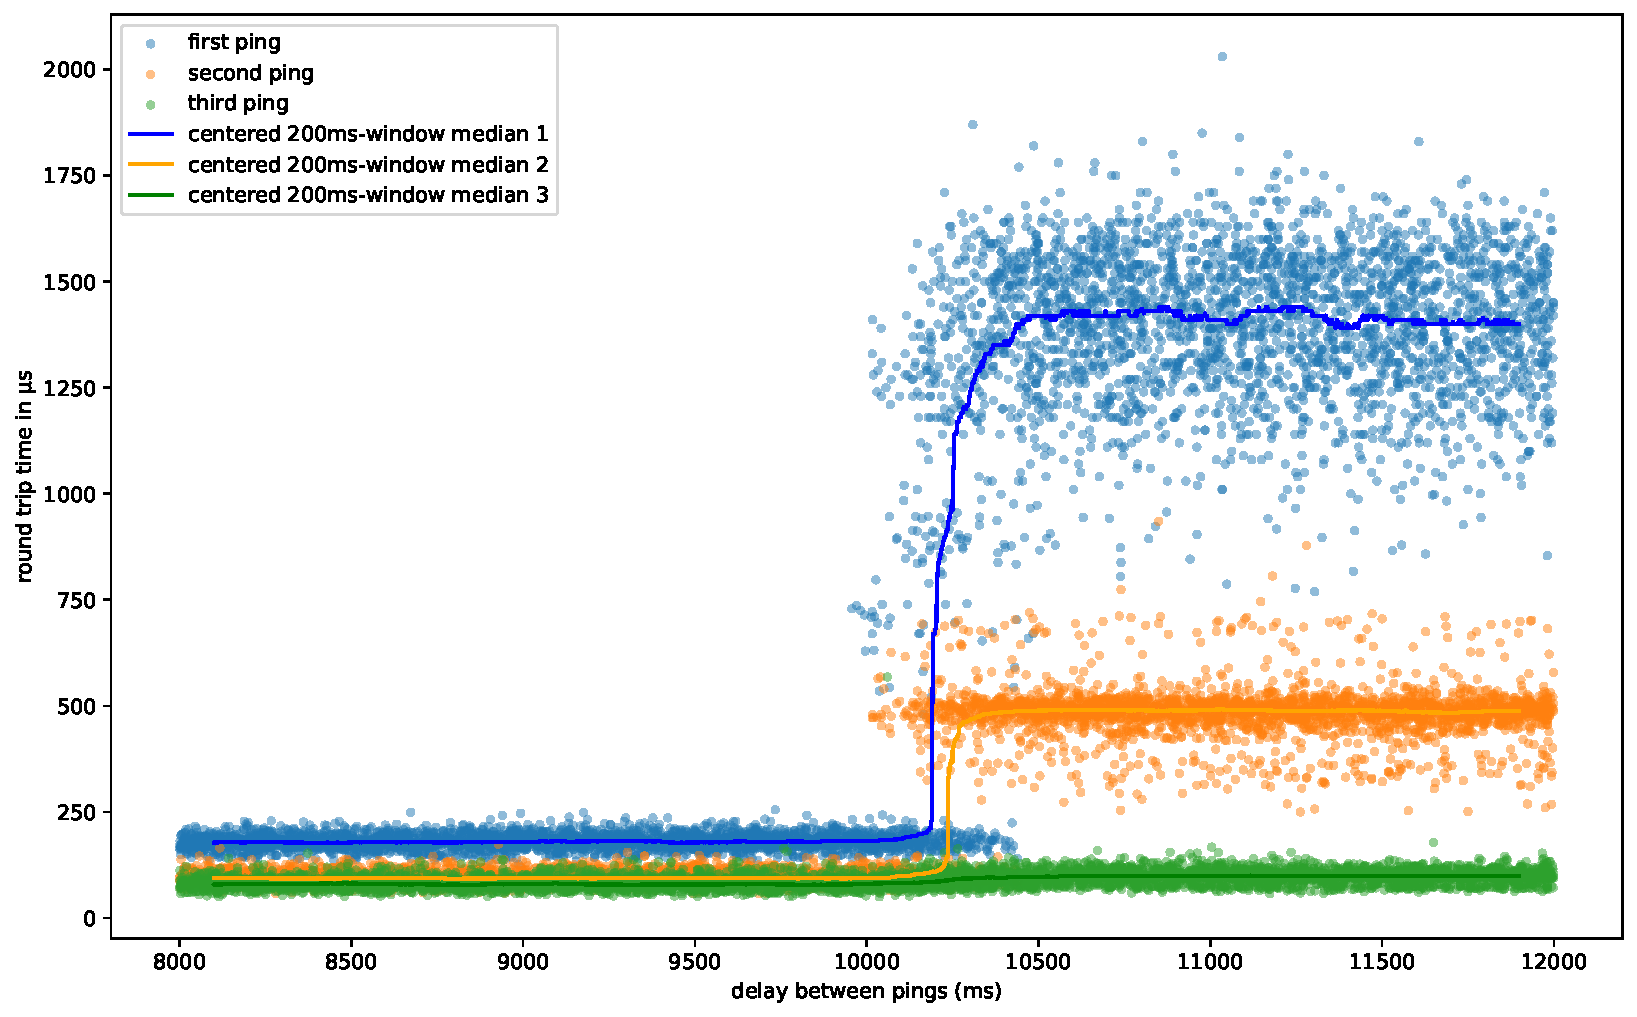
\includegraphics[width=.9\linewidth]{img/randomized_eviction_timeout.pdf}
    \caption{Results of the eviction timeout experiment with cropped outliers}
    \label{fig:plot-eviction-timeout}
\end{figure}

\paragraph{The timeout} The measured latencies of the experiment (\cref{fig:plot-eviction-timeout}) show the flow rule eviction taking effect between $10$ and $10.5$ seconds after the datapath rule installation. We assume that the timeout in software is $10$ seconds, and infrequent eviction runs cause the additional delay.

The experimental findings are consistent with the source code. In OVS's source code, the default rule timeout defined in the file \ident{ofproto/ofproto.h} as 10 seconds:
\begin{verbatim}
#define OFPROTO_MAX_IDLE_DEFAULT 10000 /* ms */
\end{verbatim}

The file \ident{ofproto/ofproto-dpif-upcall.c} contains code enforcing the timeout in the function \ident{revalidate()}:

\begin{verbatim}
if (kill_them_all || (used && used < now - max_idle)) {
    result = UKEY_DELETE;
}
\end{verbatim}

\paragraph{Difference in latency below timeout}
The results show an increased latency for the first ping compared to the second ping even when the flow rule is already installed in the datapath. We attribute this behavior to CPU caches and the internal datapath caching of rule lookups. \todo{link to explanation}


\paragraph{Increase in latency of the second ping} The measured data show another unexpected OVS behavior. The second round trip time increases when the interval is longer than the timeout by about 250 \si{\micro\second}. We do not know how to explain it.\todo{any ideas?}


\section{Cost of an upcall}
\label{res:upcall-cost}
\todo{consider joining with the previous section}

\paragraph{Cost of an upcall}
The measured data also show the cost of an upcall. The difference between round trip time without an upcall and with an upcall is around $1$ \si{\milli\second}. More precisely:
\todo{measure more samples again on dedicated hw, and maybe filter out outliers, comment on the high variance above the timeout}


% QT_QPA_PLATFORM=xcb python postprocessing/randomized_eviction_timeout.py results/randomized_eviction_timeout_2023-01-01.csv
\begin{table}[h!]
    \begin{center}
        \caption{Statistics of measured round trip times when the interval > 11 seconds}
        \label{tab:upcall-cost}
        \begin{tabular}{r|S[table-format=5.2]S[table-format=5.2]S[table-format=5.2]}
            & \textbf{First ping RTT} & \textbf{Second ping RTT} & \textbf{Difference} \\
            \hline
            \textbf{\#samples} & 359 & 359 & 359 \\
            \textbf{Mean} & 2396.82 & 1821.39 & 575.43\\
            \textbf{Std} & 6070.44 & 7258.98 & 5307.93\\
            \textbf{Min} & 1090.0 & 483.0 & -58590.0\\
            \textbf{25th percentile} & 1500.0 & 733.0 &  \\
            \textbf{Median} & 1630.0 & 674.0 & 872.0 \\
            \textbf{75th percentile} & 1730.0 & 815.0 & 993.0 \\
            \textbf{Max} & 81600.0 & 70100.0 & 28460.0 \\
        \end{tabular}
    \end{center}
\end{table}

\section{Packets generating upcalls}
\label{res:upcall-generators}
\todo{graf je netisknutelny, co se s tim da udelat?}

\begin{figure}
    \centering
    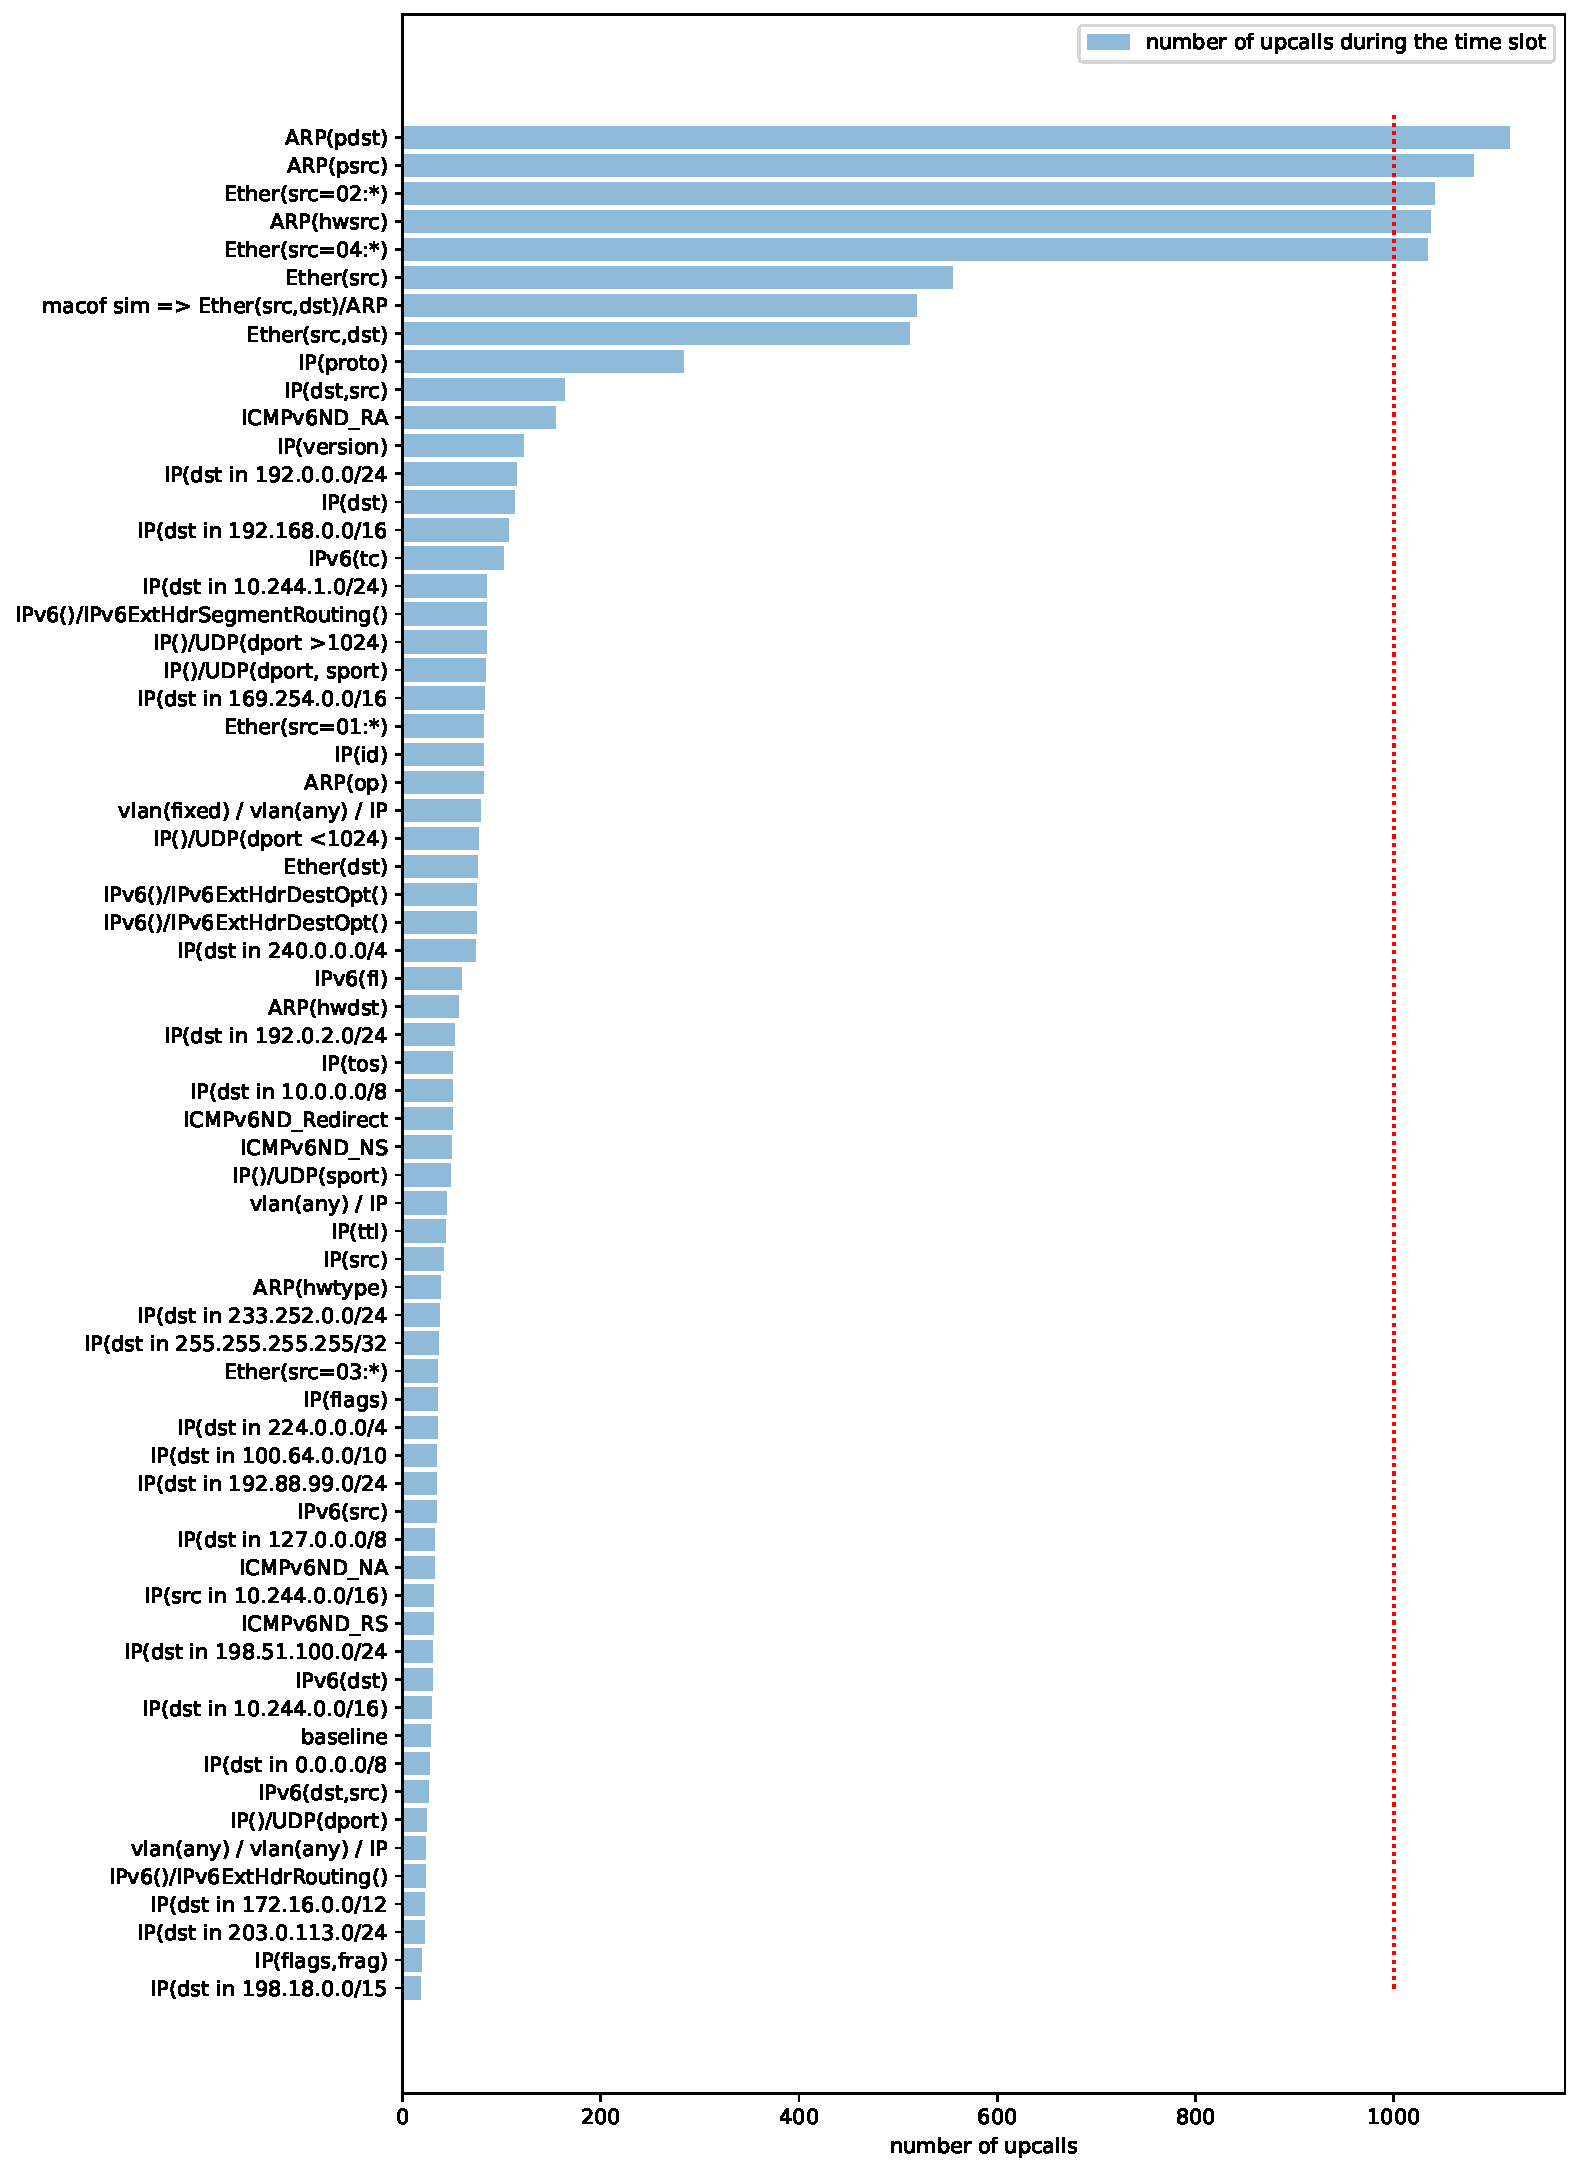
\includegraphics[width=.9\linewidth]{img/packet_fuzz.pdf}
    \caption{Number of upcalls generated by varying certain header fields in packets}
    \label{fig:plot-packet-fuzz}
\end{figure}

\Cref{fig:plot-packet-fuzz} shows the number of upcalls generated after sending 1000 crafted packets differing only in a value of a specified header field. The most significant result of this experiment is that varying Ethernet source addresses and address fields in ARP packets (except for target hardware address) generates an upcall for every packet.

\subsection{Ethernet source addresses}

Varying the Ethernet source address in the unicast range\todo{link to reference} generates new upcalls. The upcalls insert flow rules similar to the following example\footnote{dumped with \ident{ovs-dpctl dump-flows}} into the datapath:

\begin{verbatim}
recirc_id(0),in_port(9),
    eth(src=04:6a:68:88:2b:eb),eth_type(0x0800),ipv4(frag=no),
    packets:0, bytes:0, used:never, actions:drop
\end{verbatim}

OVN has a feature called port security which can be enabled for logical switch ports. By enabling port security on a port, MAC spoofing is prevented and all packets with the wrong MAC address are dropped. OVN-Kubernetes enables this feature. The command \ident{ovn-nbctl list Logical\_Switch\_Port} prints configuration for all logical switch ports, including information about port security. The following snippet is part of the command's output, a description of the logical switch port used for our test pod called \ident{arch}.

\begin{verbatim}
_uuid               : cc7a2d01-52b4-4529-a026-55bf9d46dc56
addresses           : ["0a:58:0a:f4:01:05 10.244.1.5"]
dhcpv4_options      : []
dhcpv6_options      : []
dynamic_addresses   : []
enabled             : []
external_ids        : {namespace=default, pod="true"}
ha_chassis_group    : []
mirror_rules        : []
name                : default_arch
options             : {
    iface-id-ver="40c48294-7f78-4cc0-8a74-cffd9ecec647",
    requested-chassis=wsfd-netdev65.ntdv.lab.eng.bos.redhat.com
}
parent_name         : []
port_security       : ["0a:58:0a:f4:01:05 10.244.1.5"]
tag                 : []
tag_request         : []
type                : ""
up                  : true
\end{verbatim}

Quoting the OVN documentation, section about the port security option\footnote{The documentation calls it a column, because the configuration is stored in a database colum}: \todo{link to https://www.man7.org/linux/man-pages/man5/ovn-nb.5.html}

\begin{quote}
    This column controls the addresses from which the host
    attached to the logical port (''the host'') is allowed to
    send packets and to which it is allowed to receive
    packets. If this column is empty, all addresses are
    permitted.

    Each element in the set must begin with one Ethernet
    address. This would restrict the host to sending packets
    from and receiving packets to the ethernet addresses
    defined in the logical port's port\_security column. It
    also restricts the inner source MAC addresses that the
    host may send in ARP and IPv6 Neighbor Discovery packets.
    The host is always allowed to receive packets to multicast
    and broadcast Ethernet addresses.
\end{quote}

The port security flow rules are added in OVN, in \ident{controller/lflow.c} in function \ident{consider\_port\_sec\_flows}\footnote{\url{https://github.com/ovn-org/ovn/blob/45bf9ed9dd2070a458bf384ce529e9ef62f26bd5/controller/lflow.c\#L3091-L3093}}. OVN adds multiple OpenFlow rules into multiple flow tables to implement port security.

Because OVS's datapath flow rules are much simpler than OpenFlow flow rules, there is no 1-1 mapping between them. Moreso, the datapath flow rules allow only positive matches. They can not express negative matches. Therefore, when we send packets with varying MAC addresses, \ident{ovs-vswitchd} evaluates the packets against the OpenFlow rules and finds out that the packet should be dropped. The newly generated datapath flow rule checks for the random MAC address and is not generic to match any other packets.

Looking at the problem from the other side, OVS's datapath is designed to assign packets to logical flows and execute the flow actions in as few instructions as possible. There are no precedence rules in the datapath flow table, the first matching rule is used and the order of insertion is not maintained. There are also only positive matches, no negative matches. Therefore, a single rule to drop all packets except for those with a given MAC address is impossible to construct.

\paragraph{Impossible implementation} MAC spoofing protection for a single MAC address can be implemented using 48 rules\todo{potentially not true, what about recirculation?}, each checking for a single flipped bit in the Ethernet address compared to the allowed address. All other rules in the flow table would have to check for a matching MAC address to prevent rule overlaps. With multiple allowed Ethernet addresses, the number of rules to drop the invalid packets would grow significantly and all other rules would have to be specified as many times as there are allowed MAC addresses.

However, to implement the protection as described, \ident{ovs-vswitchd} would have to know that MAC spoofing protection is desired. OVN (or any other SDN) configures OVS through OpenFlow rules which can not express negative matches either. The MAC spoofing protection is therefore implemented as several linked rule tables with explicit rule priorities and rule actions resubmitting the packets to different tables. Therefore, \ident{ovs-vswitchd} can not easily infer the intention and translate the flow rules properly.

% translation happens here https://github.com/openvswitch/ovs/blob/64cdc290ef441bc3b4c2cddc230311ba58bc31b3/ofproto/ofproto-dpif-xlate.c#L7769-L7778
% struct xlate_in https://github.com/openvswitch/ovs/blob/64cdc290ef441bc3b4c2cddc230311ba58bc31b3/ofproto/ofproto-dpif-xlate.h#L66
% struct xlate_ctx https://github.com/openvswitch/ovs/blob/64cdc290ef441bc3b4c2cddc230311ba58bc31b3/ofproto/ofproto-dpif-xlate.c#L195

\subsection{ARP packet fields}

ARP packets with varying hardware addresses behave the same as ordinary Ethernet packets with varying source hardware addresses because port security in OVN applies to them as well. The reason why this can not be easily fixed is also the same.

\subsection{Other types of packets}

\xxx{Shouldn't Neighbor discovery packets cause the same as they are blocked by the port security? How are multicast packets not causing upcalls?}

\section{Impact of upcall heavy traffic}

\subsection{Standard behavior}
\label{subsec:standard-behavior}

\begin{figure}
    \centering
    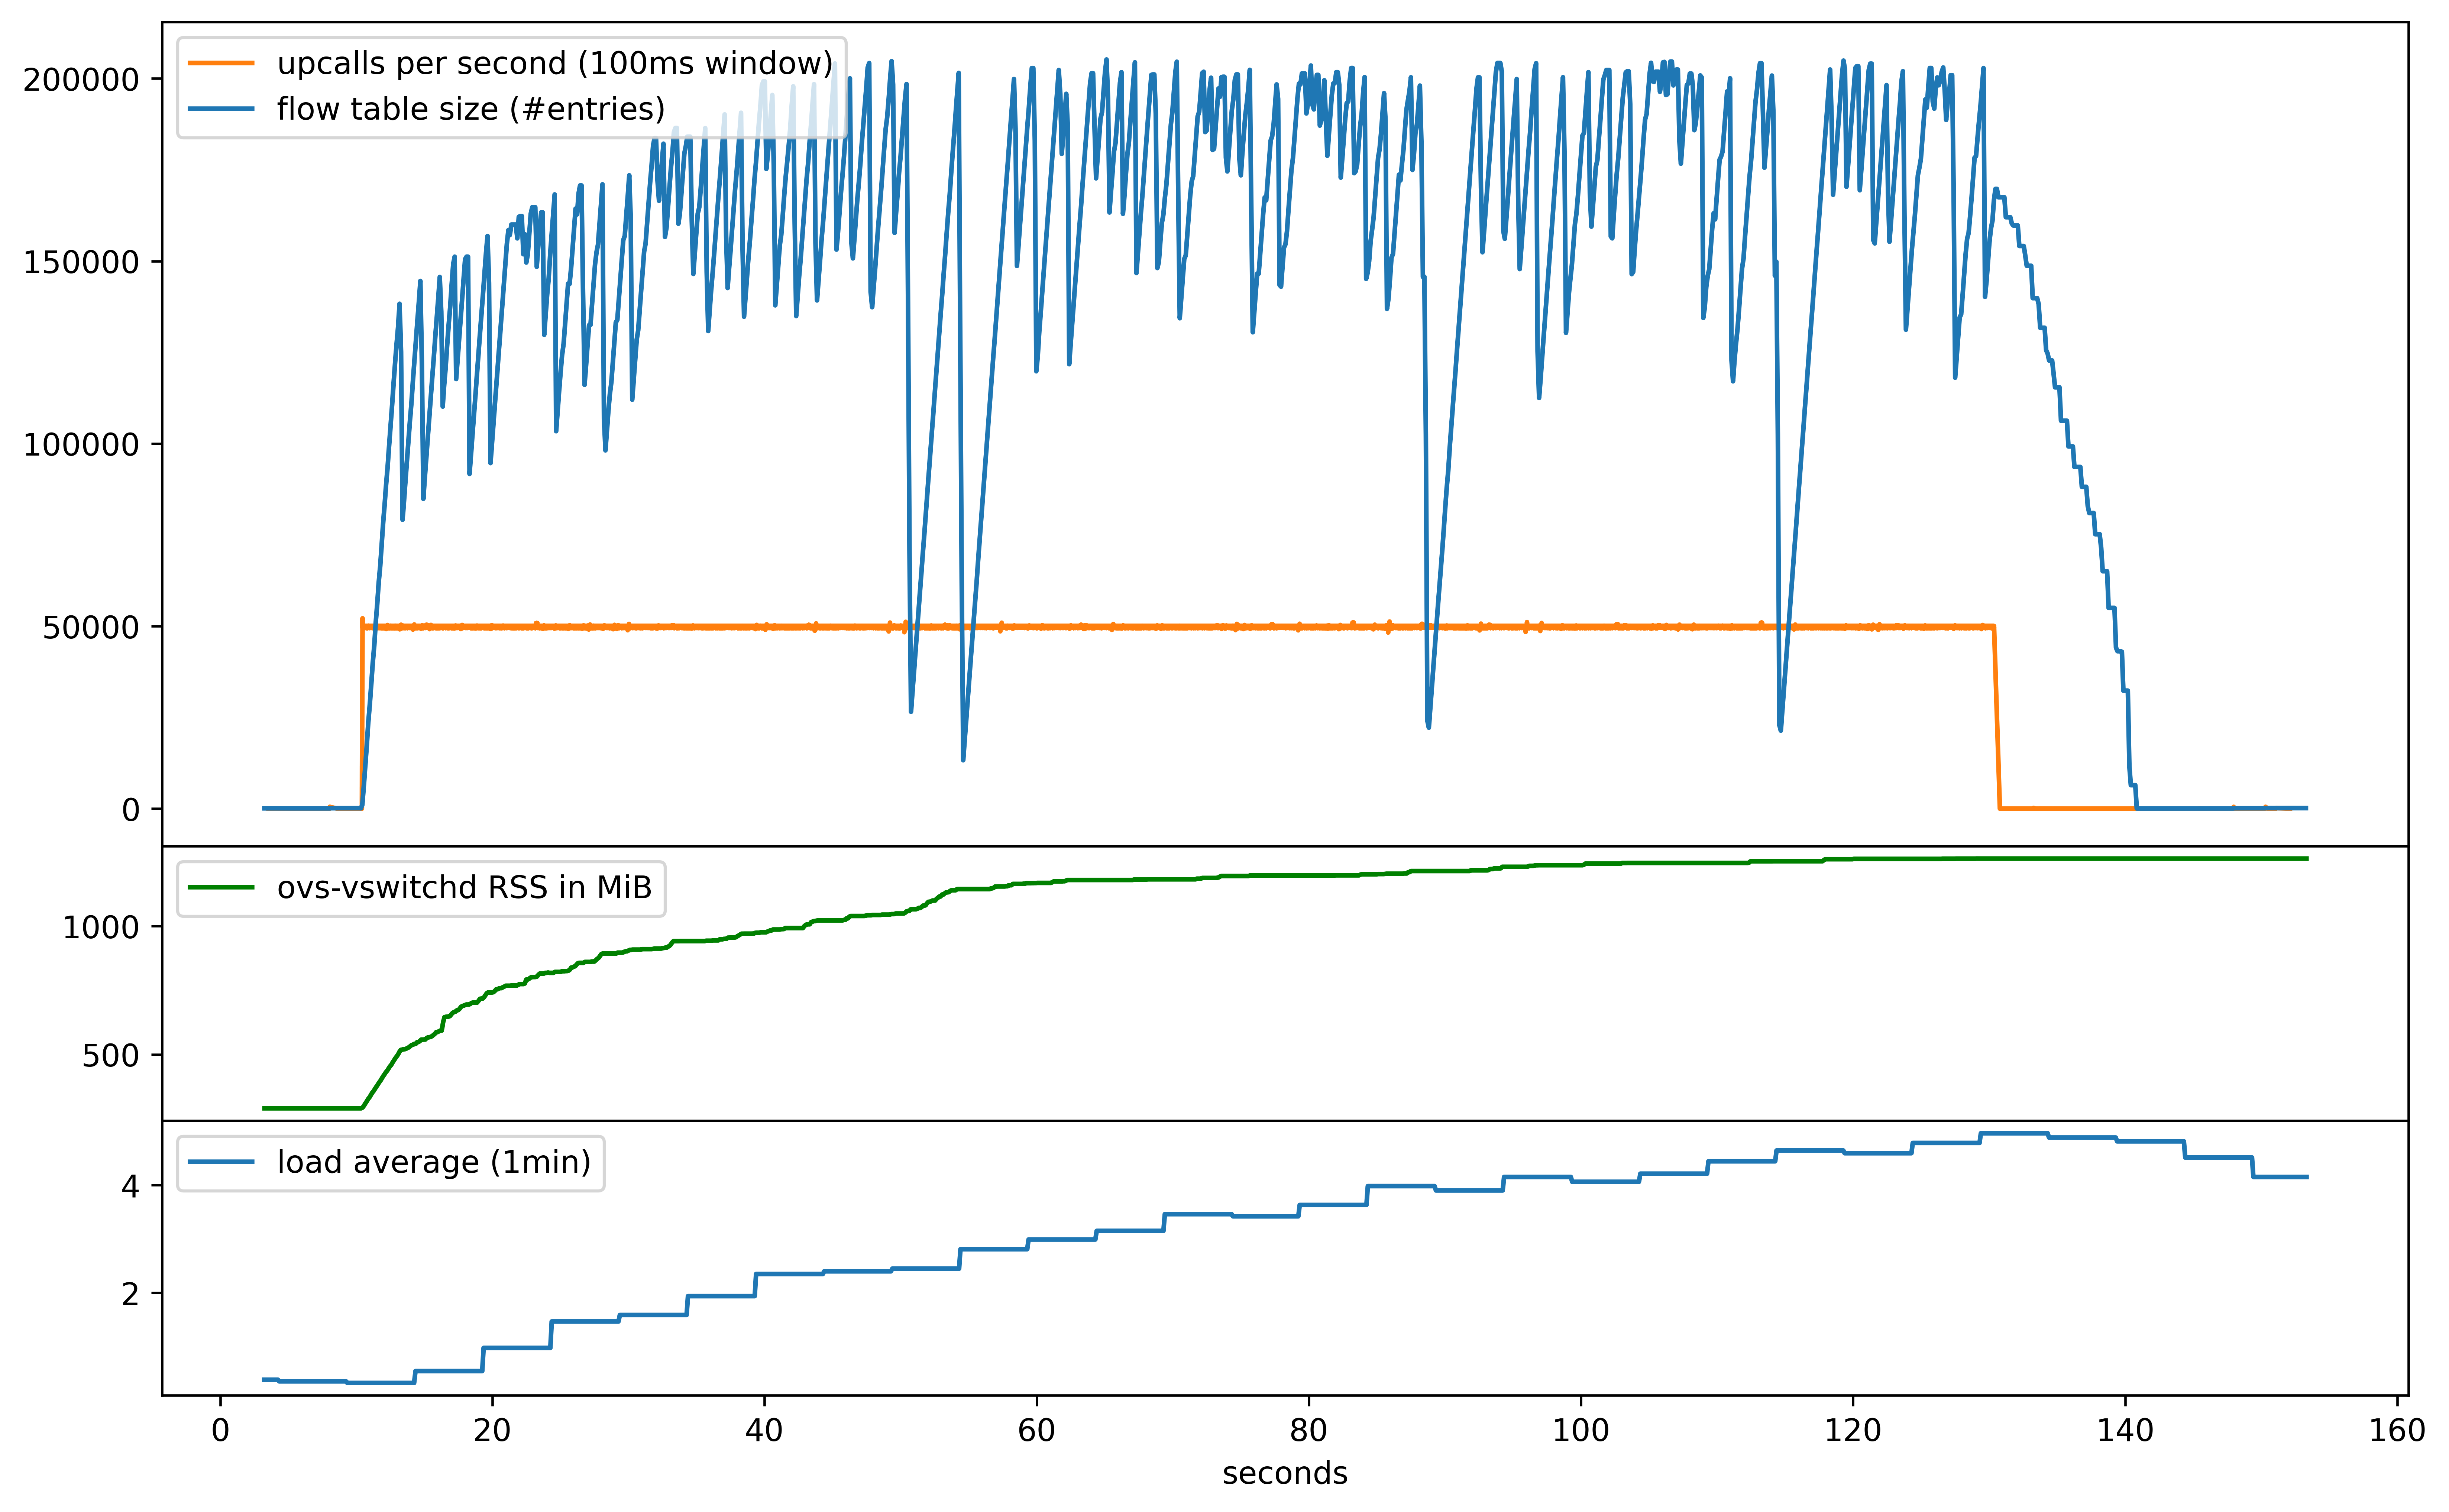
\includegraphics[width=.9\linewidth]{img/packet_flood_bare_50k.png}
    \caption{\ident{ovs-vswitchd} stressed with 50k upcalls per second}
    \label{fig:plot-packet-flood-bare-50k}
\end{figure}

\begin{figure}
    \centering
    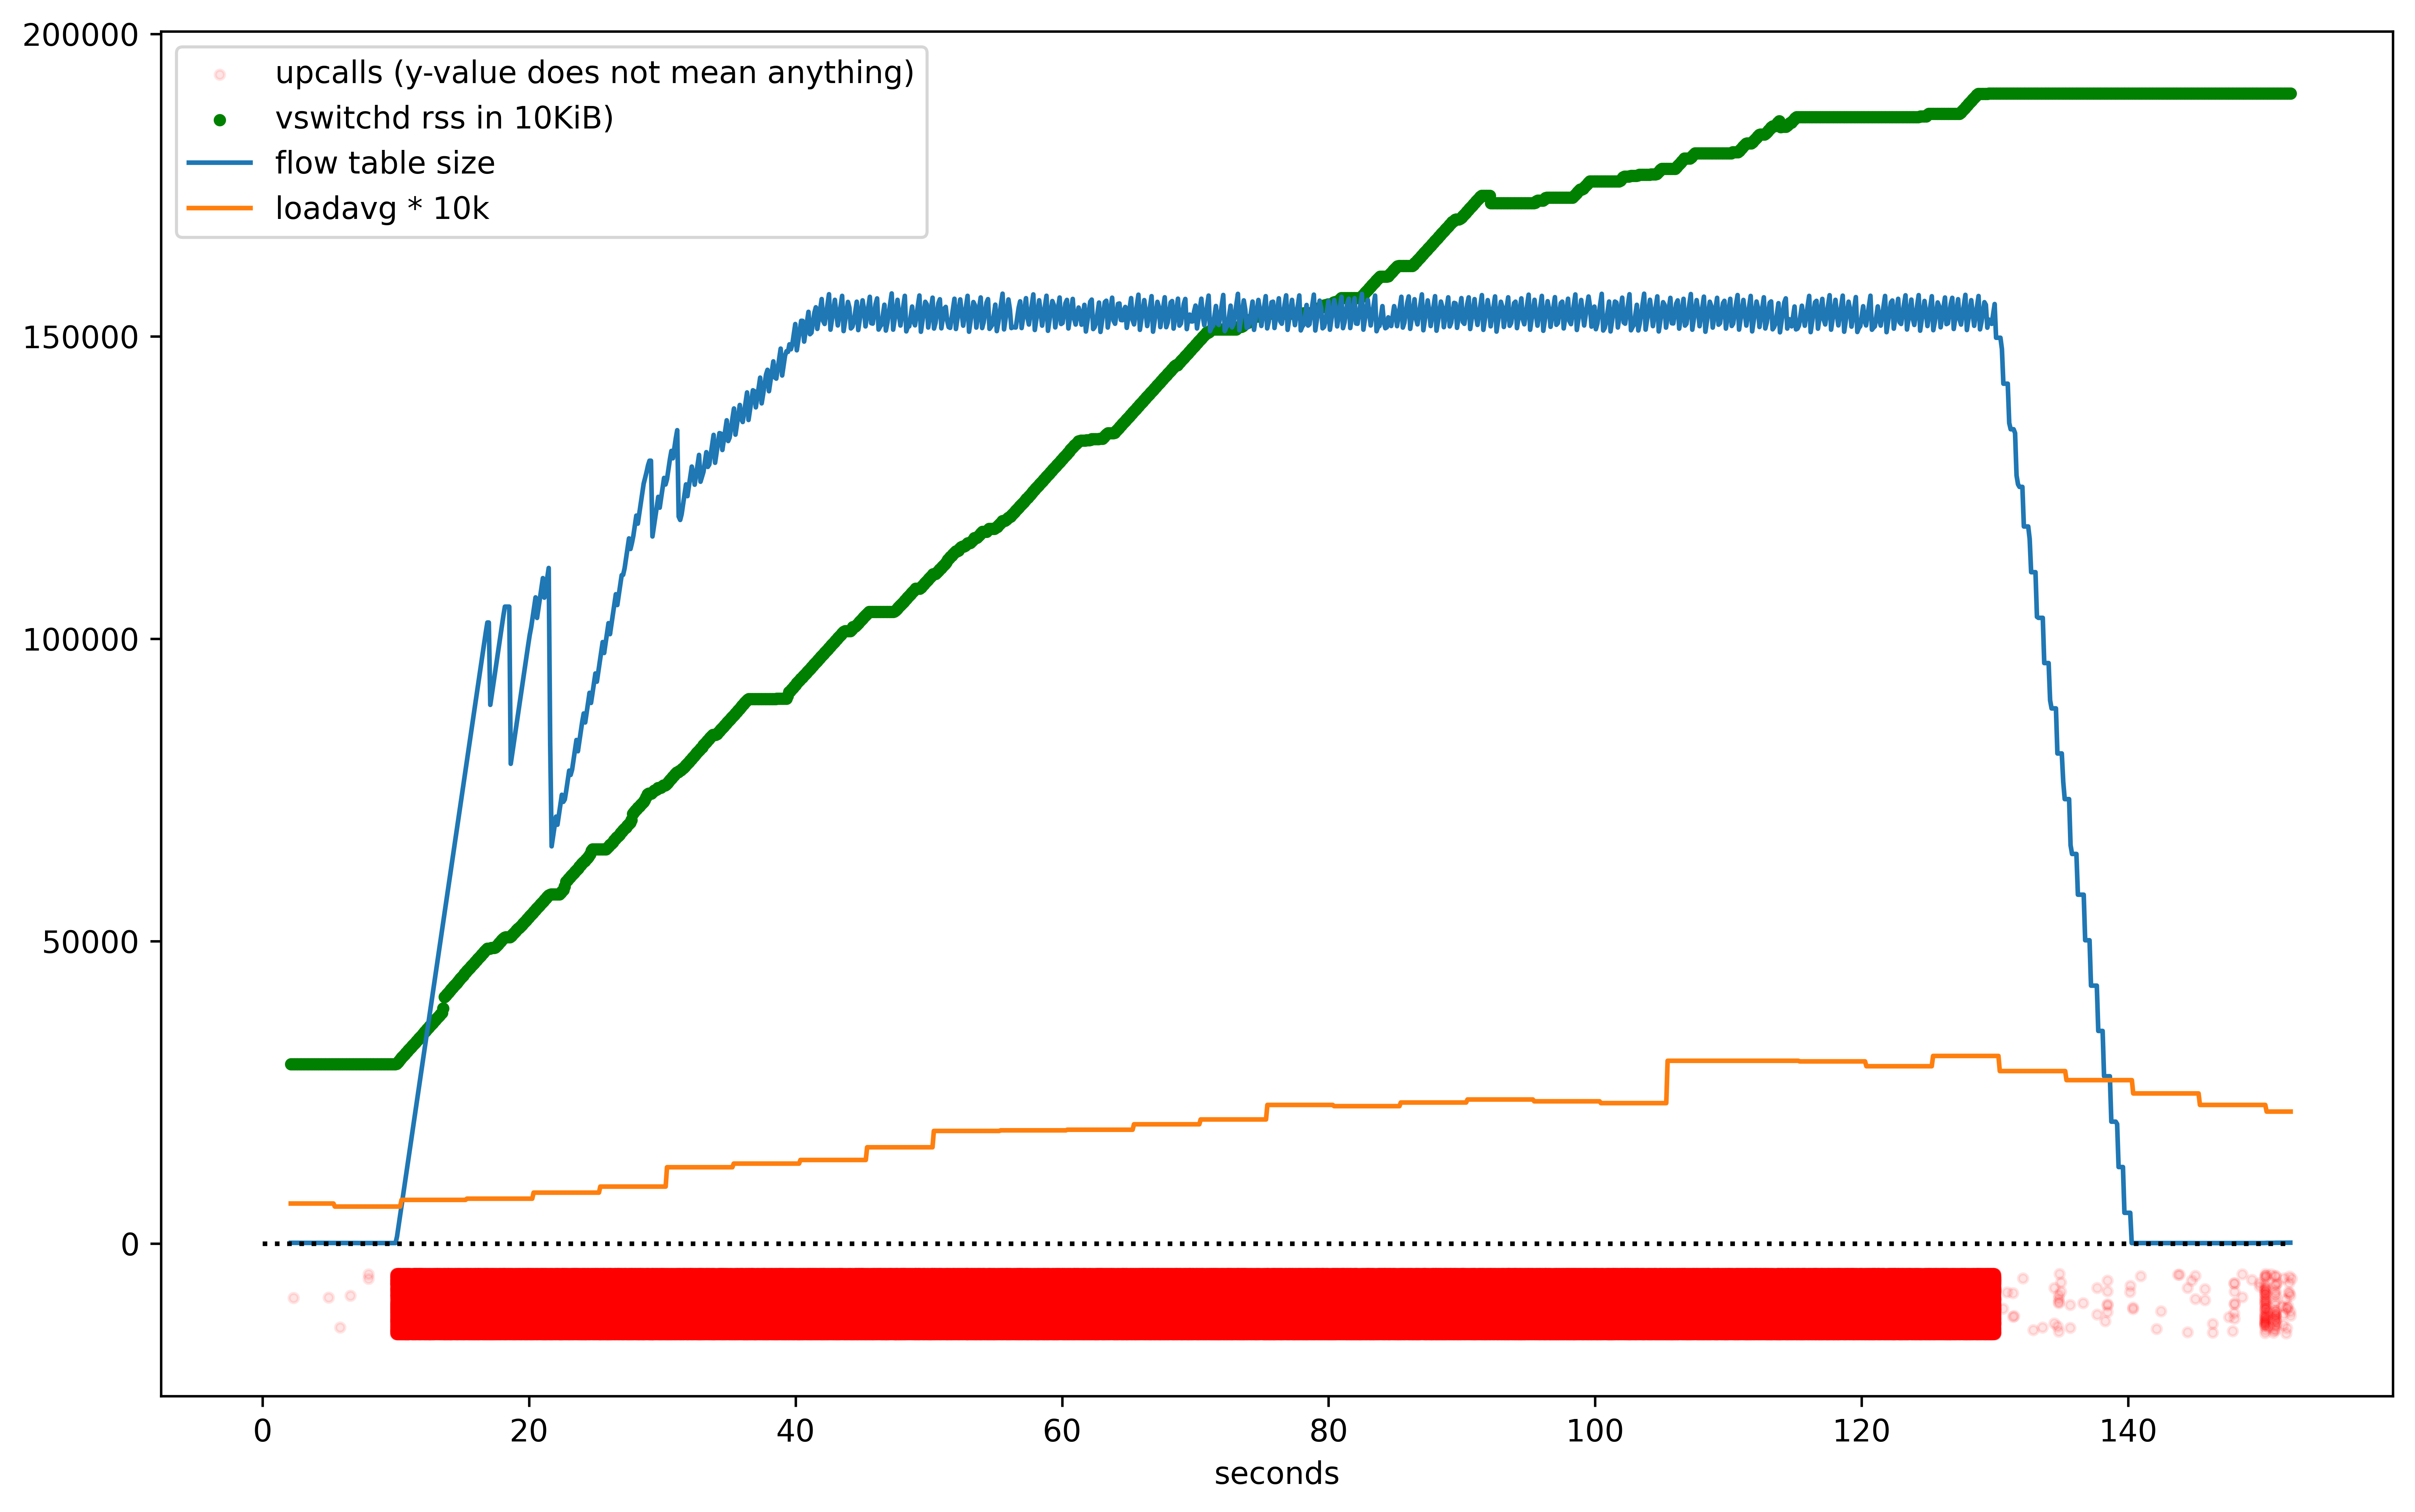
\includegraphics[width=.9\linewidth]{img/packet_flood_bare_15k.png}
    \caption{\ident{ovs-vswitchd} stressed with 15k upcalls per second}
    \label{fig:plot-packet-flood-bare-15k}
\end{figure}

\todo{in experiment design, note that we always test with freshly restarted vswitchd}

\paragraph{Flow table size}
\Cref{fig:plot-packet-flood-bare-50k} and \cref{fig:plot-packet-flood-bare-15k} show recorded behavior of \ident{ovs-vswitchd} when stressed with significant number of upcalls. Assuming the 10-second flow rule timeout would be the only criteria for evicting flow rules, the flow tables should have reached 500k and 150k flow rules respectively. However, \ident{ovs-vswitchd} has a default limit\todo{link to source} of 200k flow rules in the table which explains the lower-than-expected table size in \cref{fig:plot-packet-flood-bare-50k}. Moreso, the flow table size limit is dynamic based on system performance\todo{link to the future} and 200k is only a hard limit beyond which the table won't ever grow. The slow increase until the hard limit is reached is visible at the beginning of \cref{fig:plot-packet-flood-bare-50k}.

In both experiments, the flow table size fluctuates. With fewer upcalls, when only the timeout is at play, the fluctuations are small and can be explained by periodic timeout enforcement in the revalidator\todo{je někde vysvětlená architektura vswitchd?} threads in \ident{ovs-vswitchd}.\todo{link to source} When the flow table size hits the 200k limit, an additional regulatory mechanism in the revalidator threads activates. Quoting a comment\footnote{\url{https://github.com/openvswitch/ovs/blob/474a179aff6c4199d8007910e3f79f000af9d659/ofproto/ofproto-dpif-upcall.c\#L2771-L2782}} from OVS's source code:

\begin{quote}
    In normal operation we want to keep flows around until they have
    been idle for 'ofproto\_max\_idle' milliseconds.  However:

    \begin{itemize}
        \item If the number of datapath flows climbs above 'flow\_limit', drop that down to 100 ms to try to bring the flows down to the limit.

        \item If the number of datapath flows climbs above twice 'flow\_limit', delete all the datapath flows as an emergency measure.  (We reassess this condition for the next batch of datapath flows, so we will recover before all the flows are gone.)
    \end{itemize}
\end{quote}

In other words, the revalidator thread checks flow rules in batches and whenever the flow table grows above the limit, a shorter timeout is applied to the current batch. We hypothesize that the high amplitude of the fluctuations is caused by synchronization between multiple threads. There are multiple revalidator threads, each has its flow rule dump thread\footnote{\url{https://github.com/openvswitch/ovs/blob/474a179aff6c4199d8007910e3f79f000af9d659/ofproto/ofproto-dpif-upcall.c\#LL2751C16-L2751C16}} and the actual rule deletion is handled in the kernel after receiving a deletion command over a netlink socket which has an internal queue. We did not confirm nor disprove the hypothesis.

\paragraph{Upcalls}
In both \cref{fig:plot-packet-flood-bare-50k} and \cref{fig:plot-packet-flood-bare-15k}, the red dots at the bottom represent individual upcalls. We have randomized their position on the y-axis to improve legibility and better visualize upcall frequency.

Whenever our stress tool runs, the red bar becomes saturated and dense. Our tool tries to send packets in regular intervals, so the red bar should appear mostly homogeneous. At the end of the test, we report the results over the network and our tools are not perfectly synchronized, hence small upcall clusters at the end of the experiment are to be expected.

In \cref{fig:plot-packet-flood-bare-50k}, we can see a lot of upcalls happen before the stress test starts and they do not appear to be happening afterwards. We do not know what is causing it.\todo{FALSE! We know!} An ICMP and UDP latency test is running in the background (results in \todo{link do sekce s latenci}) as well as an SSH connection, but these packets should not be causing a significant number of upcalls. Furthermore, if it were caused by these packets, it should have continued after the stress test had finished. The other experiment shown here in \cref{fig:plot-packet-flood-bare-15k} has these upcalls both before and after the stress test. In other tests, we have also observed no extra upcalls.

\paragraph{System load}
Our packet flooding tool is a single-threaded application and therefore directly contributes to the load averages only by a value of 1 or less. The current limit of our stress test tool running on the dedicated servers is roughly 200k packets per second on a single CPU core. However, we observe a significantly higher load average in both recorded experiments, in \cref{fig:plot-packet-flood-bare-50k} and in \cref{fig:plot-packet-flood-bare-15k}. Except for our experiment, the system is idle. Hence we attribute the additional system load to OVS. As we discussed before\todo{where?}, OVS uses multiple threads during normal operation. By default, the revalidator threads iterate over the whole flow table every 500 \si{\milli\second} and command the kernel to delete flow rules. The upcall handlers continuously translate OpenFlow rules to datapath rules and command the kernel to insert new flow rules. All of this busy work causes an extra system load.

Worryingly though, the additional system load is not attributed to the process causing it. Containers or virtual machines on hosts using OVS can cause additional system load outside of their allowance.

\paragraph{Memory usage}
In both \cref{fig:plot-packet-flood-bare-50k} and \cref{fig:plot-packet-flood-bare-15k}, the resident set size of \ident{ovs-vswitchd} increases and stabilizes at slightly less than 2GB. The allocated memory is never released and stays allocated even after the flooding stops. The used memory seems to be proportional to the flow table size.

Same as with the system load, memory usage bypasses resource accounting. A container or a VM with minimal resource allowance can use more resources than the system administrators configured.

\subsection{Impact on latency}

\begin{figure}
    \centering
    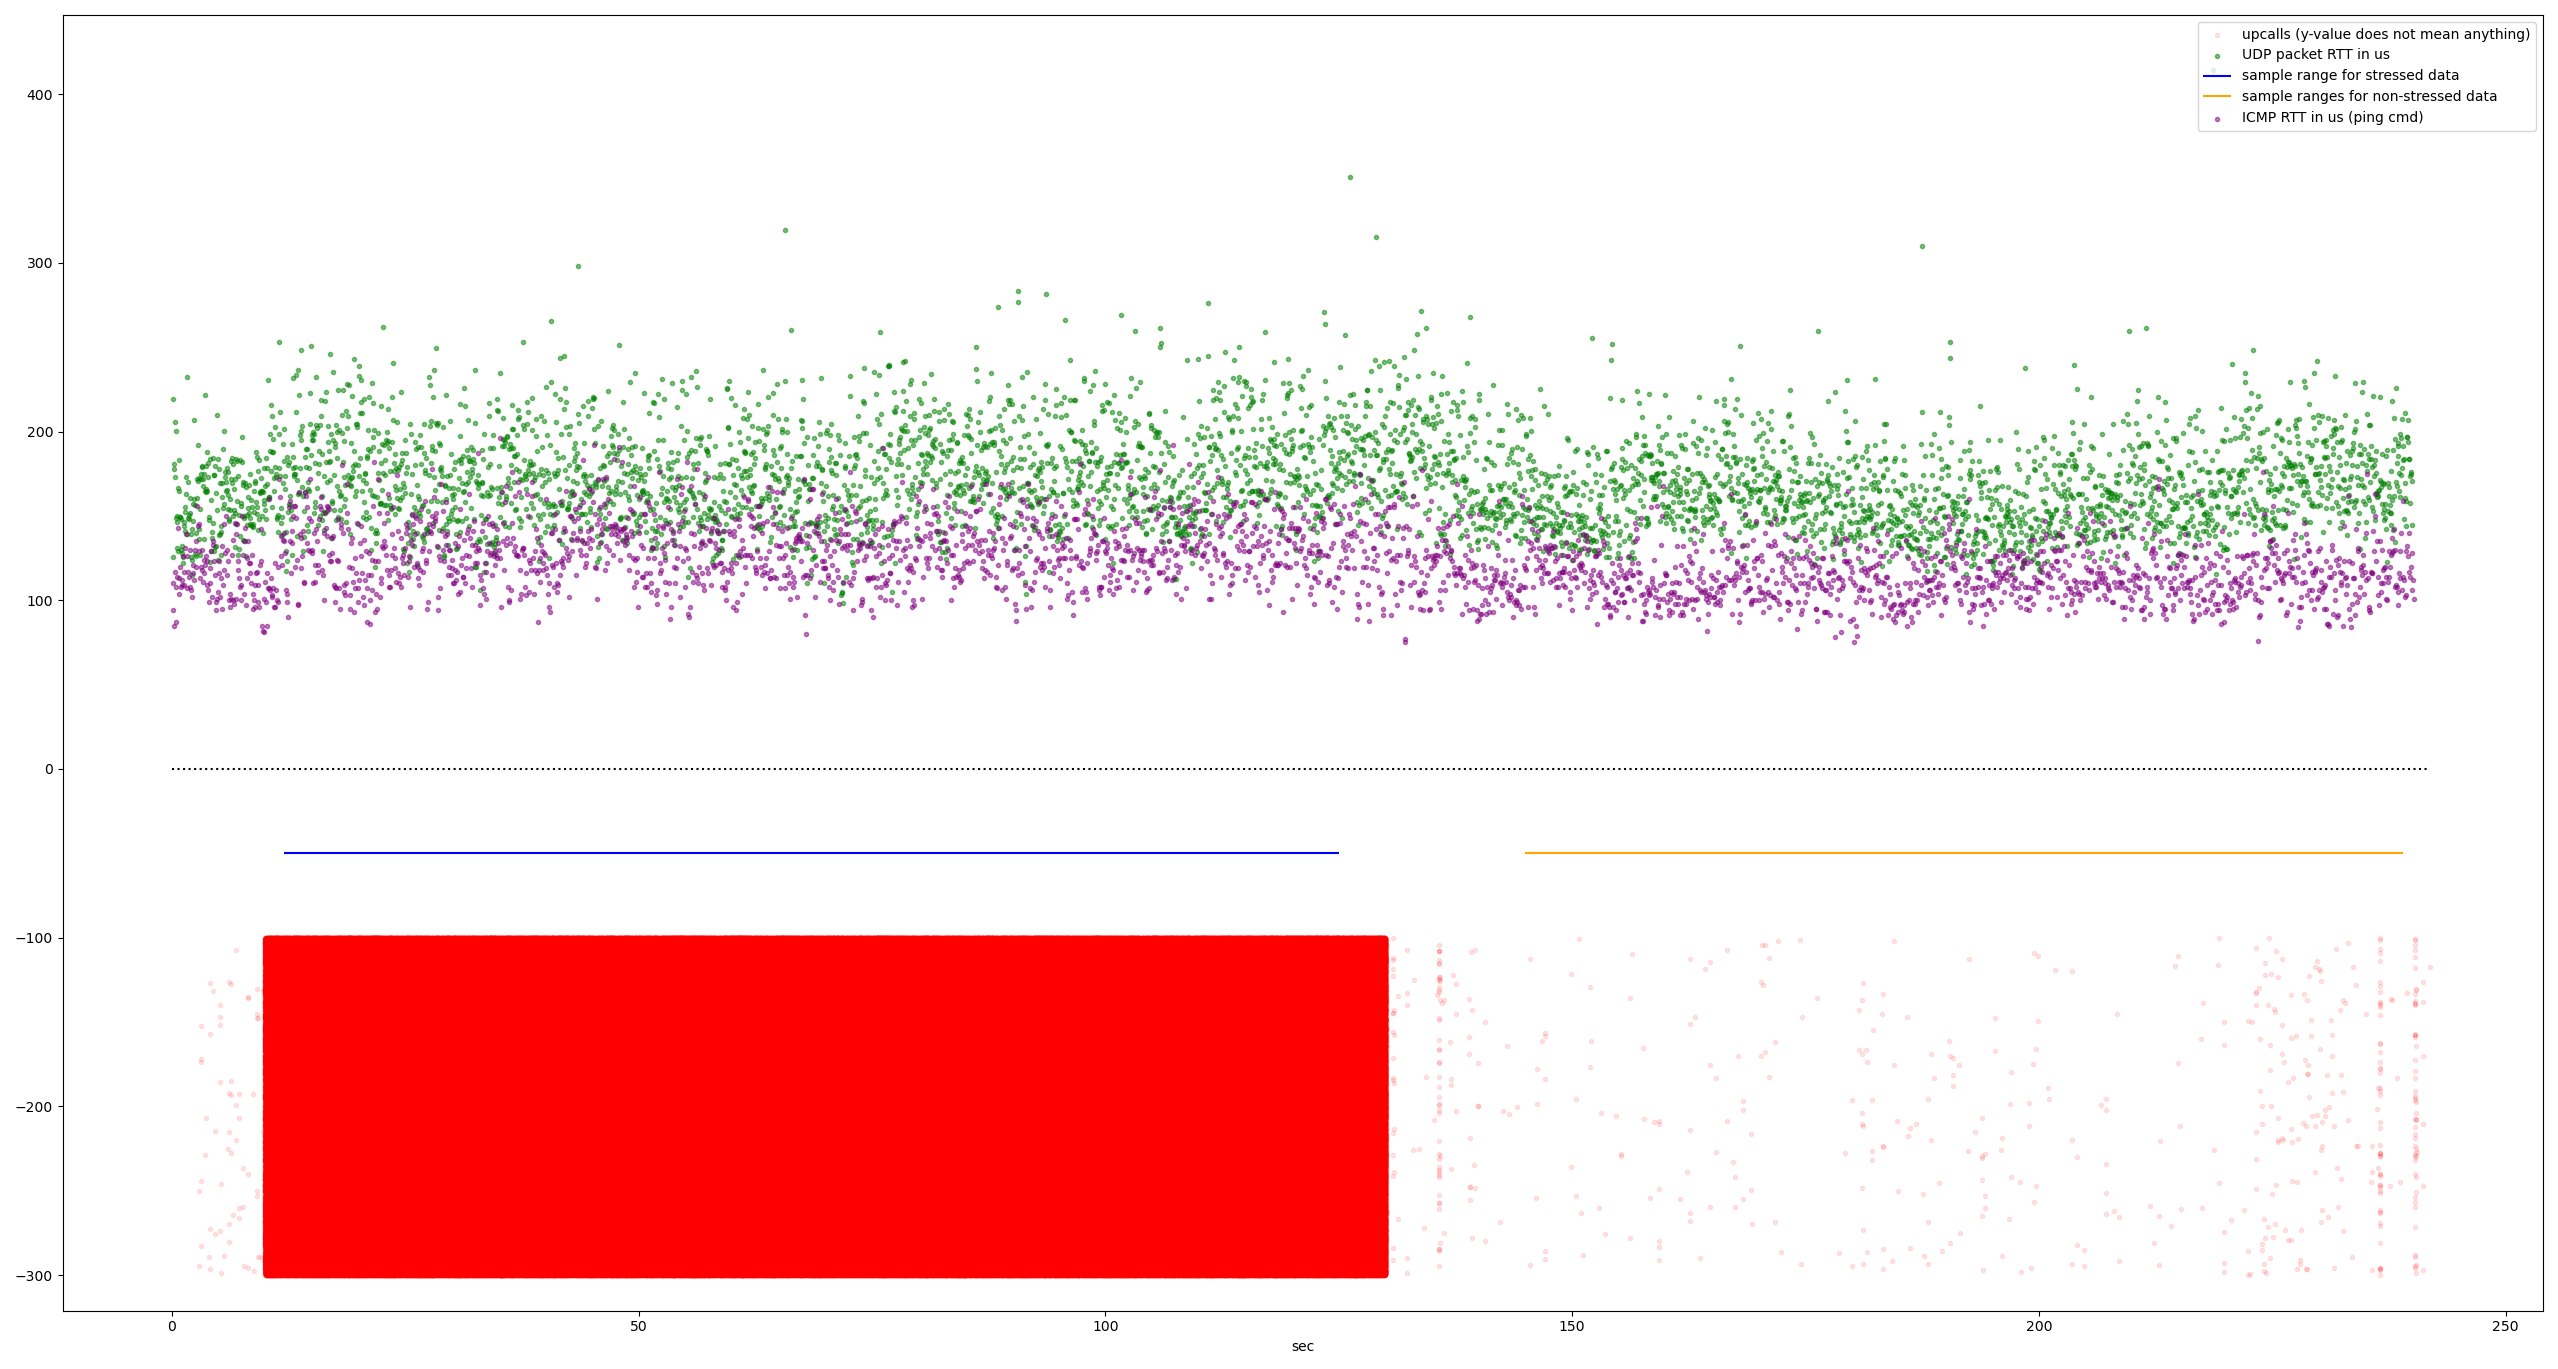
\includegraphics[width=.9\linewidth]{img/packet_flood_50k_latency.png}
    \caption{Round trip times during 50k upcalls/sec stress test}
    \label{fig:plot-packet-flood-50k-latency}
\end{figure}

\Cref{fig:plot-packet-flood-50k-latency} shows the results of a different run of the same experiment. The plot shows only the latencies measured from the \ident{victim}\todo{describe the test architecture} pod. The ICMP tests target the node IP address of \kb{1}, the UDP tests target the node IP address of \kb{3}. The horizontal lines mark the ranges of samples used for a statistical test.

While there does not seem to be any practically significant difference between stressed and non-stressed system in the round-trip-times, the difference is statistically significant. Considering only the UDP-based results, there are $2255$ samples in the stressed range with a mean value of $175980 \pm 1320$ \si{\nano\second}\footnote{$95\%$ confidence interval, assuming normal distribution}. The non-stressed range has 1876 samples and a mean value of $164404 \pm 1174$ \si{\nano\second}. The difference between the means is $11576$ \si{\nano\second}.

% stressed UDP latency
% shape: (9, 3)
% ┌────────────┬────────────┬───────────────┐
% │ describe   ┆ ts         ┆ latency_ns    │
% │ ---        ┆ ---        ┆ ---           │
% │ str        ┆ f64        ┆ f64           │
% ╞════════════╪════════════╪═══════════════╡
% │ count      ┆ 2255.0     ┆ 2255.0        │
% │ null_count ┆ 0.0        ┆ 0.0           │
% │ mean       ┆ 68.502237  ┆ 175980.142794 │
% │ std        ┆ 32.628849  ┆ 31963.391742  │
% │ min        ┆ 12.025217  ┆ 98250.0       │
% │ max        ┆ 124.979466 ┆ 762959.0      │
% │ median     ┆ 68.502056  ┆ 173259.0      │
% │ 25%        ┆ 40.238689  ┆ 155156.0      │
% │ 75%        ┆ 96.765862  ┆ 193006.0      │
% └────────────┴────────────┴───────────────┘
% (175980.14279379157, 174660.18226166346, 177300.10332591968)
% non-stressed UDP latencies
% shape: (9, 3)
% ┌────────────┬────────────┬───────────────┐
% │ describe   ┆ ts         ┆ latency_ns    │
% │ ---        ┆ ---        ┆ ---           │
% │ str        ┆ f64        ┆ f64           │
% ╞════════════╪════════════╪═══════════════╡
% │ count      ┆ 1876.0     ┆ 1876.0        │
% │ null_count ┆ 0.0        ┆ 0.0           │
% │ mean       ┆ 191.99893  ┆ 164404.665245 │
% │ std        ┆ 27.143008  ┆ 25925.644717  │
% │ min        ┆ 145.023486 ┆ 107262.0      │
% │ max        ┆ 238.975234 ┆ 495776.0      │
% │ median     ┆ 191.999098 ┆ 161704.5      │
% │ 25%        ┆ 168.52374  ┆ 146410.0      │
% │ 75%        ┆ 215.52409  ┆ 178624.0      │
% └────────────┴────────────┴───────────────┘
% (164404.66524520254, 163230.7366655189, 165578.5938248862)


\section{Performance when resource limited}

In \cref{subsec:standard-behavior}, we talked about extra memory and CPU usage of /ident{ovs-vswitchd}. The default containerized deployment of OVN-Kubernetes limits\footnote{https://github.com/ovn-org/ovn-kubernetes/blob/b982b8cadba939c55010829f61eb5ebe4fd90794/dist/templates/ovs-node.yaml.j2\#L84-L90} \ident{ovs-vswitchd} to 400 MiB of physical memory and two-tenths of a single CPU core. In the remainder of this section, when we write about limiting memory or CPU, we mean using Kubernetes to enforce the resource limit just as the default containerized deployment does it.

\subsection{Memory limit}
We tried limiting only the memory usage of \ident{ovs-vswitchd}, leaving the CPU time unlimited. When we flooded the system with upcalls, \ident{ovs-vswitchd} crashed without leaving any meaningful error message behind. During normal operations, everything seemed normal.

We tried to limit the number of flow rules using the following command:
\begin{verbatim}
ovs-vsctl set Open_vSwitch . other_config:flow-limit=10000
\end{verbatim}

The limit somewhat helps and when the upcall frequency is not too high (double or triple the limit), everything works. However, once we flood the network with even more packets, the flow limit is overshot and \ident{ovs-vswitchd} again crashes.

Our theory is that the crash happens during the revalidator dump phase, when \ident{ovs-vswitchd} makes a copy of all in-kernel flow rules in the userspace. This allocates more memory than allowed and the container is subsequently terminated:

\begin{quote}
    A Container can exceed its memory request if the Node has memory available. But a Container is not allowed to use more than its memory limit. If a Container allocates more memory than its limit, the Container becomes a candidate for termination. If the Container continues to consume memory beyond its limit, the Container is terminated. If a terminated Container can be restarted, the kubelet restarts it, as with any other type of runtime failure.
    \todo{link source https://kubernetes.io/docs/tasks/configure-pod-container/assign-memory-resource/}
\end{quote}


\subsection{CPU limit}

When CPU bound, \ident{ovs-vswitchd} does not crash. It tries to do the opposite and dynamically change the datapath's flow rule limit based on the revalidator thread's performance.\todo{link to source} We can see the effect in \cref{fig:packet-flood-limited}.

\begin{figure}
    \centering
    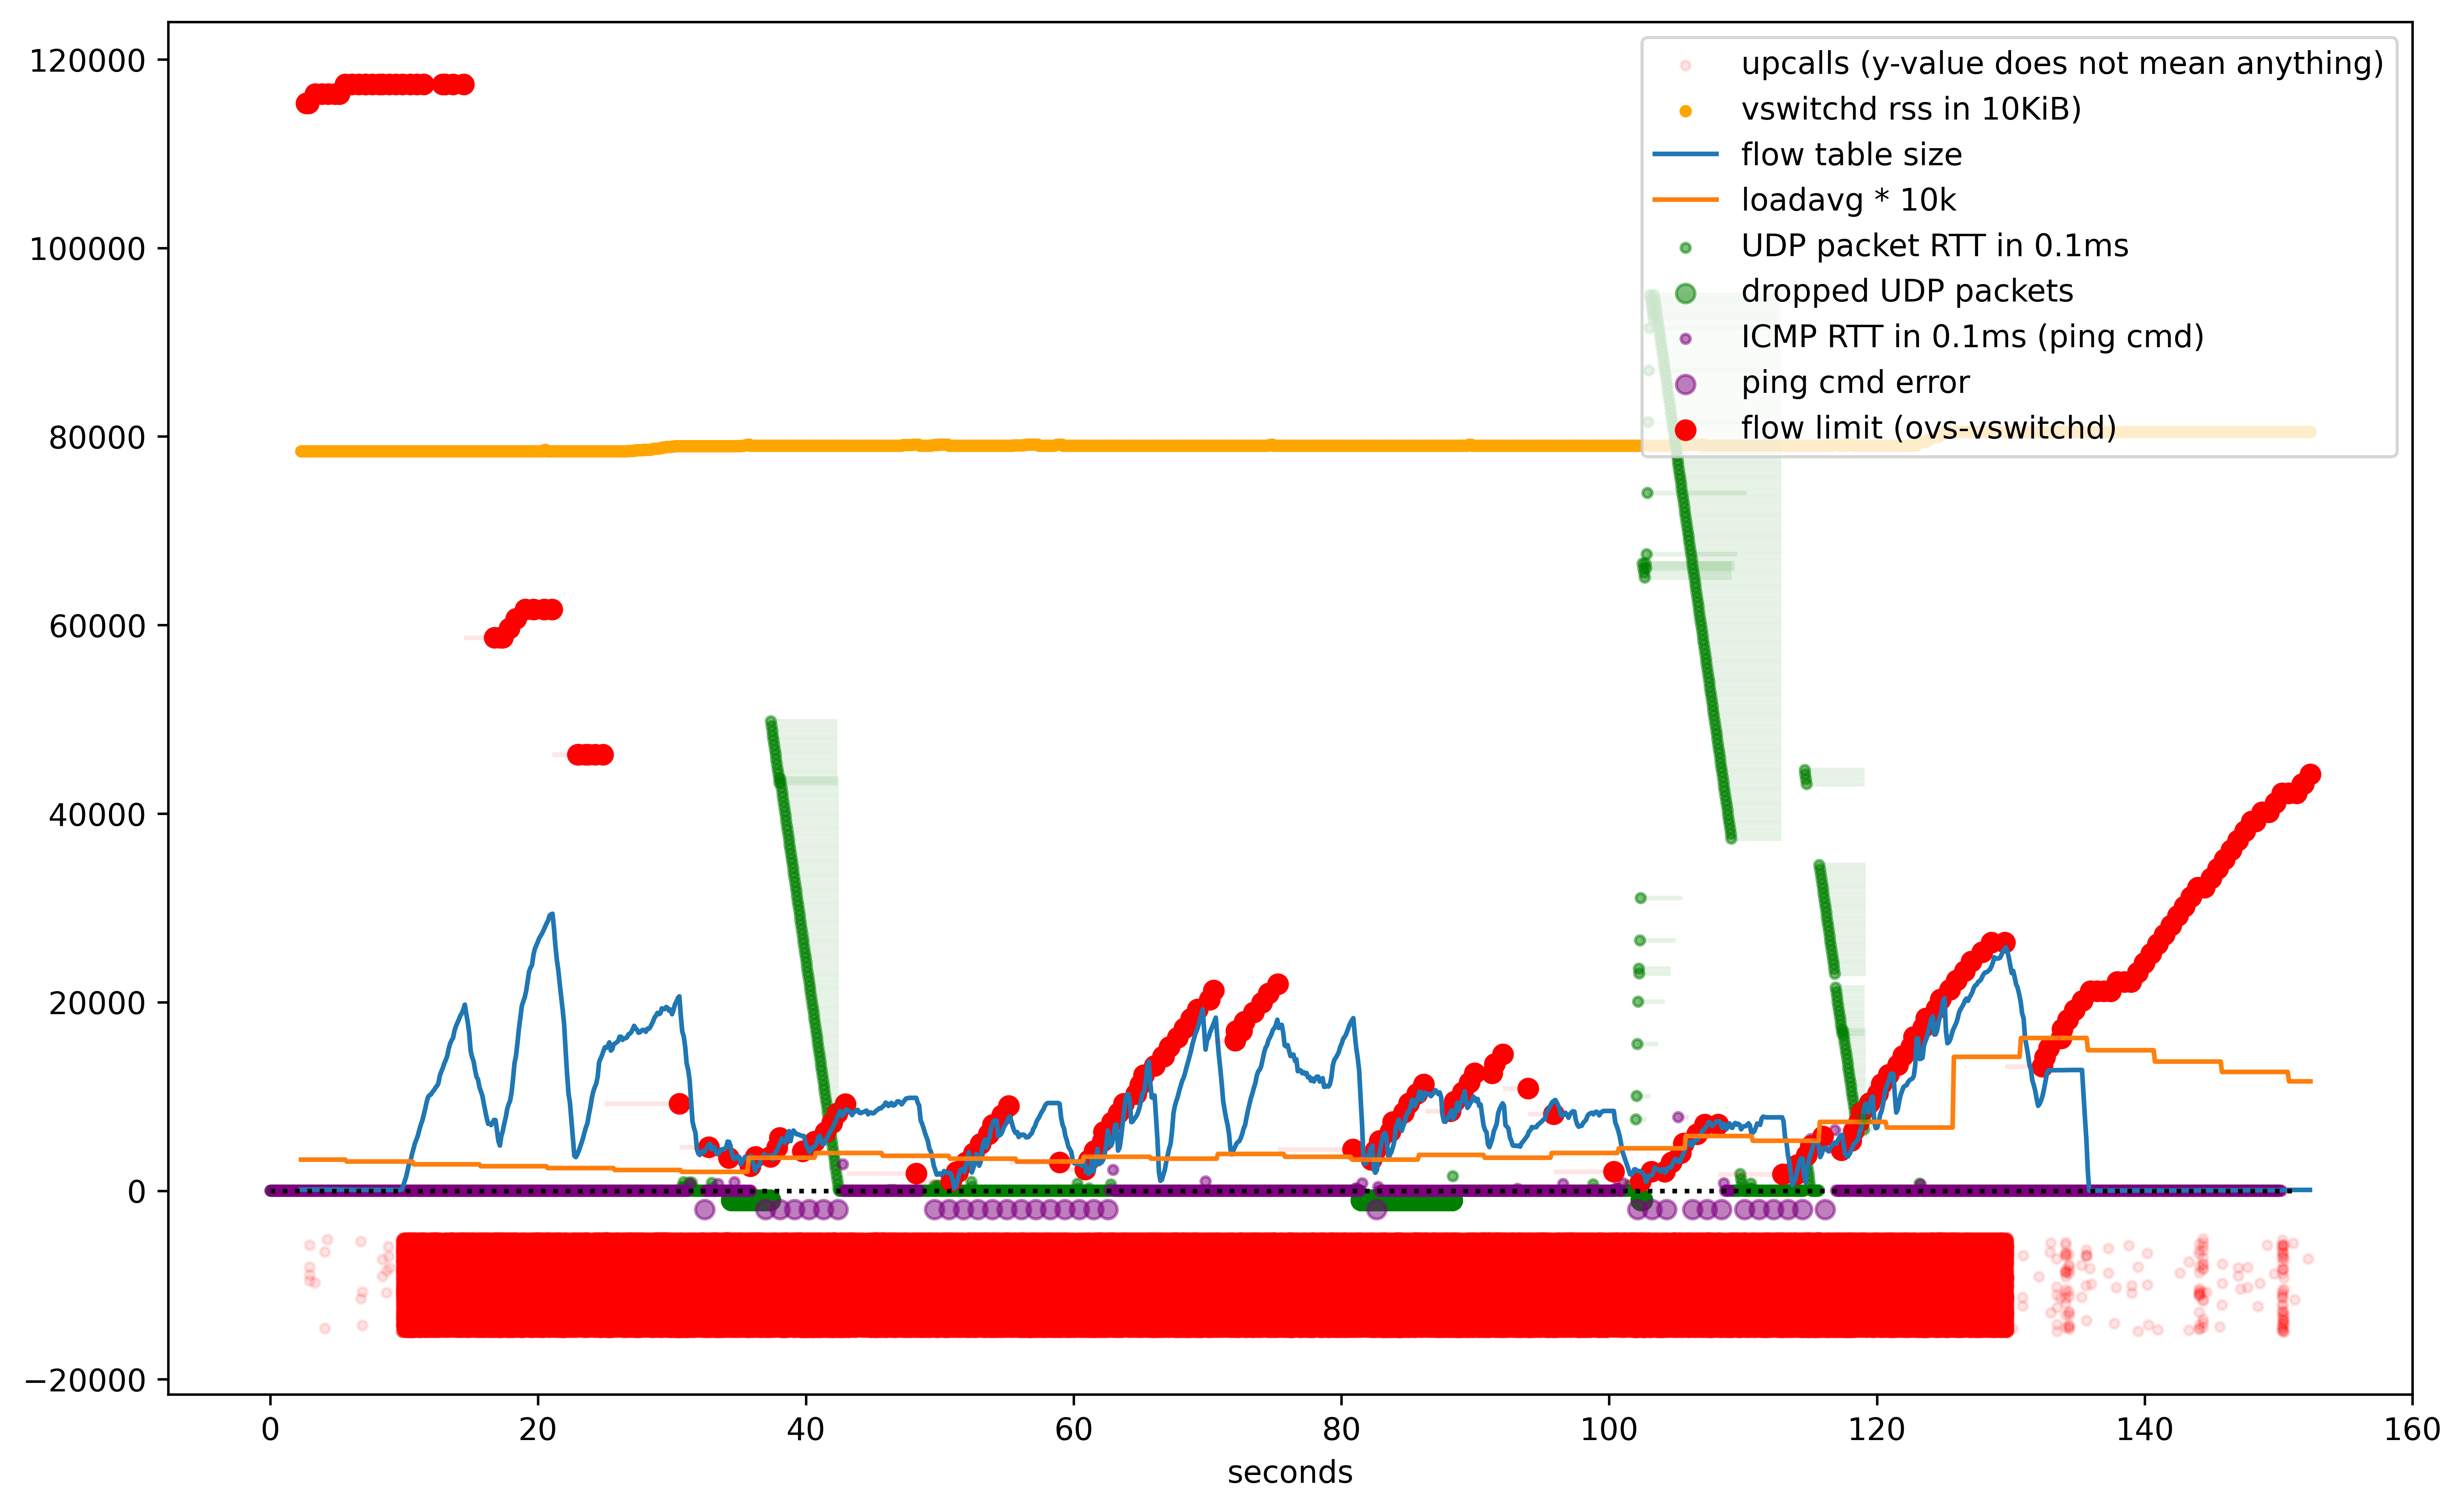
\includegraphics[width=.9\linewidth]{img/packet_flood_limited_resources_50k.png}
    \caption{5k upcalls/sec stress test}
    \label{fig:packet-flood-limited}
\end{figure}

When compared to the previous experiments:

\begin{itemize}
    \item The rate of upcalls is only $5000$ per second, $\frac{1}{10}$ of the experiments before.
    \item Memory usage stays almost constant.
    \item Load average (1 minute) peaks at the value 2, but stays below 1 most of the time.
    \item The size of the datapath flow table varies a lot more. We can see the same higher frequency variations as before, but now they are combined with lower frequency variations created by the dynamically changing flow limit.
    \item Latency measurements are added to the plot (beware of the unusual units). They are the same as when we talked about latency before, now combined in a single experiment. The highest round-trip-time observed is around 10 seconds long. Sometimes, sending a packet completely fails (indicated by thicker dots below the number line).
\end{itemize}


\section{Accidental bug discovery}
\todo{this is really a placeholder with the email I wrote, replace it with something meaningful...}

Hi,

I think I might have found a bug or just a really weird unexpected behavior. I am reporting it here, but I've reproduced it only on systems with OVN-Kubernetes and OVN. I don't know whether it can be replicated with standalone OVS.


\subsection{Test environment}


3 node Kubernetes cluster using OVN-Kubernetes, Docker and Fedora 38. All nodes in a single LAN with IPs 192.168.1.{221,222,223}. From now on, I will refer to the nodes only by the last digit of their IP address.


\subsection{Steps to reproduce:}


\begin{enumerate}
\item install a pod with a shell and a ping command (I am using docker.io/archlinux:latest, always running on node 222)
\item run `kubectl exec -ti \$POD\_NAME -- ping 192.168.1.221`
\item in a different terminal, ssh into the host of the pod (in my case node 222) and run `ovs-dpctl del-flows`
\item observe the measured latencies
\item keep the ping running and kill ovs-vswitchd on the host and wait for its restart
\item observe the latencies
\end{enumerate}


\subsection{What I observe}


\begin{verbatim}
[root@wsfd-netdev64 ~]# kubectl exec -ti arch -- ping 192.168.1.221
PING 192.168.1.221 (192.168.1.221) 56(84) bytes of data.
64 bytes from 192.168.1.221: icmp_seq=1 ttl=63 time=0.543 ms
64 bytes from 192.168.1.221: icmp_seq=2 ttl=63 time=0.160 ms
64 bytes from 192.168.1.221: icmp_seq=3 ttl=63 time=0.119 ms
64 bytes from 192.168.1.221: icmp_seq=4 ttl=63 time=0.144 ms
64 bytes from 192.168.1.221: icmp_seq=5 ttl=63 time=0.137 ms
64 bytes from 192.168.1.221: icmp_seq=6 ttl=63 time=0.996 ms  # < ovs-dpctl del-flows
64 bytes from 192.168.1.221: icmp_seq=7 ttl=63 time=0.808 ms
64 bytes from 192.168.1.221: icmp_seq=8 ttl=63 time=1.01 ms
64 bytes from 192.168.1.221: icmp_seq=9 ttl=63 time=1.24 ms
64 bytes from 192.168.1.221: icmp_seq=10 ttl=63 time=1.20 ms
64 bytes from 192.168.1.221: icmp_seq=11 ttl=63 time=1.14 ms
64 bytes from 192.168.1.221: icmp_seq=12 ttl=63 time=1.10 ms  # < killall ovs-vswitchd
  From 10.244.1.5 icmp_seq=22 Destination Host Unreachable
  From 10.244.1.5 icmp_seq=23 Destination Host Unreachable
  From 10.244.1.5 icmp_seq=24 Destination Host Unreachable
  From 10.244.1.5 icmp_seq=25 Destination Host Unreachable
  From 10.244.1.5 icmp_seq=26 Destination Host Unreachable
  From 10.244.1.5 icmp_seq=27 Destination Host Unreachable
  From 10.244.1.5 icmp_seq=28 Destination Host Unreachable
  From 10.244.1.5 icmp_seq=29 Destination Host Unreachable
  From 10.244.1.5 icmp_seq=31 Destination Host Unreachable
  From 10.244.1.5 icmp_seq=32 Destination Host Unreachable
64 bytes from 192.168.1.221: icmp_seq=34 ttl=63 time=1371 ms
64 bytes from 192.168.1.221: icmp_seq=35 ttl=63 time=322 ms
64 bytes from 192.168.1.221: icmp_seq=36 ttl=63 time=0.186 ms
64 bytes from 192.168.1.221: icmp_seq=37 ttl=63 time=0.192 ms
64 bytes from 192.168.1.221: icmp_seq=38 ttl=63 time=0.140 ms
64 bytes from 192.168.1.221: icmp_seq=39 ttl=63 time=0.163 ms
^C
--- 192.168.1.221 ping statistics ---
39 packets transmitted, 18 received, +10 errors, 53.8462% packet loss, time 38769ms
rtt min/avg/max/mdev = 0.119/94.570/1370.551/318.102 ms, pipe 3
\end{verbatim}

After flushing the datapath flow rules, the RTTs increase. This indicates an upcall for every single packet. I confirmed this by tracing the kernel and the upcalls are definitely there (actually, this is how I discovered the whole issue). The system can remain in this state for a long time (at least minutes).

After restarting vswitchd, the upcalls stop happening and everything is fast again.


I have also confirmed, that the same thing happens to UDP packets. The same also happens regardless of which node in the cluster I target, even the pod's host.


\subsection{What I expect}


I expected only a few upcalls in response to flushing the datapath, after which a new datapath rules would get inserted into the kernel.


\subsection{Repeatability}


Flushing the rules and restarting vswitchd seems to be a certain method to flip the system between the two different states. However the upcall-making state seems unstable and it sometimes reverts back to the expected lower-latency state by itself. It appears to me that flooding the system with unrelated upcalls and rules increases the chance of an "autonomous fix".


At this point, I don't believe this would cause significant problems. I just find the behavior extremely weird.

Is there something more I could provide to help with reproducing this? Or should I report it elsewhere?


Best,
Vašek Šraier 

\section{Lock contention investigation}
\todo{write about the fact, that there does not seem to be a problematic lock in OVS, because we checked them almost all}